% Modified for use with IJQC - Madhusudan Singh Copyright (C) (2011). All rights reserved.
\documentclass[12pt]{article}

\setlength{\oddsidemargin}{0in}  %left margin position, reference is one inch
\setlength{\textwidth}{6.5in}    %width of text=8.5-1in-1in for margin
\setlength{\topmargin}{-0.5in}    %reference is at 1.5in, -.5in gives a start of about 1in from top
\setlength{\textheight}{9in}     %length of text=11in-1in-1in (top and bot. marg.) 
\newenvironment{wileykeywords}{\textsf{Keywords:}\hspace{\stretch{1}}}{\hspace{\stretch{1}}\rule{1ex}{1ex}}

\usepackage{amsmath,amssymb}
\usepackage{graphicx}% Include figure files
\usepackage{caption}
\usepackage{bm}
\usepackage{color}% Include colors for document elements
\usepackage{dcolumn}% Align table columns on decimal point
\usepackage[numbers,super,comma,sort&compress]{natbib}

\usepackage{soul}

\definecolor{background-color}{gray}{0.98}
\graphicspath{{data/}{images/}}

%\title{Atomic pseudo-potentials for sp$^2$ carbon atoms}
\title{Atomic pseudo-potentials for reproducing $\pi$-orbital electron behaviour in sp$^2$ carbon atoms}
\author{Alexander Punter, Paola Nava, Yannick Carissan \thanks{Aix-Marseille Universit\'e, CNRS, Centrale Marseille, iSm2, Marseille, France}}

\begin{document}

\maketitle

\begin{abstract}
A pseudo-potential system for an sp\(^{2}\) carbon atom is built and tested as a building block for various pseudo-hydrocarbon polyenes and polycyclic aromatic hydrocarbons.  
This pseudo-system has a central charge of $Z=1$, it contains only one electron.
It is employed in \textsl{ab-initio} calculations in which several physical characteristics 
including the orbital energies and first ionisation energy, as well as first excitation energy and UV spectra, are found to be well-reproduced by the pseudo-system. 
Remarkably, not only are the $\pi$ excitation energies in good agreement with the reference calculations, but also transition
densities and intensities, confirming that the virtual space obtained with the pseudo-potentials is of excellent quality.
Finally, this approach is capable of reproducing the $\pi$ electron systems of small or large, planar hydrocarbons at low computational cost.
\end{abstract}

\begin{wileykeywords}
Pseudo-potentials, $sp^2 carbon$, PAH, aromaticity, $\pi$ system.
\end{wileykeywords}

\clearpage
% 
% \begin{figure}[h]
% \centering
% \colorbox{background-color}{
% \fbox{
% \begin{minipage}{1.0\textwidth}
% 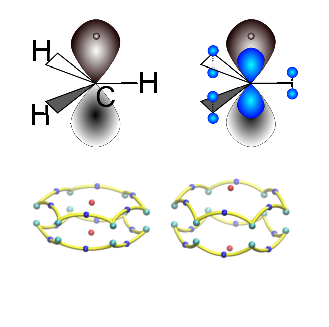
\includegraphics[width=50mm,height=50mm]{graphical_abstract.eps} % Pick only one of the two styles by uncommenting the corresponding \includegraphics
% %\includegraphics[width=110mm,height=20mm]{cc.eps}
% A pseudo-potential system for an sp\(^{2}\) carbon atom is built and tested as a building block for various pseudo-hydrocarbon polyenes and polycyclic aromatic hydrocarbons.  
% It is employed in \textsl{ab-initio} calculations in which several physical characteristics are found to be well-reproduced by the pseudo-system. 
% This approach is capable of reproducing the $\pi$ electron systems of planar hydrocarbons at low computational cost.
% \\
% \end{minipage}
% }}
% \end{figure}


\makeatletter
\renewcommand\@biblabel[1]{#1.}
\makeatother

\bibliographystyle{apsrev}

\renewcommand{\baselinestretch}{1.5}
\normalsize

\clearpage

%%BEGTXT
\section*{\sffamily \Large INTRODUCTION}

Since Hellmann and Gomb\'as' development of the first pseudo-potentials in the 1930s,\cite{hellmann_1935, gombas_1935} pseudo-potential methods have been employed in a variety of theoretical chemistry problems. In recent years, pseudo-potentials have been used to provide enhancements or corrections to other methods, with examples including their use as link atoms in QM/MM calculations,%
\cite{%
singh_combined_1986,
assfeld_quantum_1996,
goedecker_separable_1996,
gao_generalized_1998,
hartwigsen_relativistic_1998,
zhang_pseudobond_1998,
dilabio_simple_2002,
von_lilienfeld_variational_2004,
von_lilienfeld_optimization_2004,
zhang_improved_2004,
von_lilienfeld_performance_2005,
dilabio_efficient_2005,
jacob_calculation_2006,
parks_pseudobond_2008,
lewin_modified_2008,
ihrig_specific_2011,
von_lilienfeld_force_2013,
hitzenberger_probing_2015,
collins_energy-based_2015,
pezeshki_recent_2015,
chung_oniom_2015,
hitzenberger_optimizing_2016} or the efforts to use them alongside DFT calculations in correcting for DFT errors in the effect of van der Waals forces.\cite{dilabio_2008} Their primary use, however, has always been that of increasing computational efficiency as compared with all-electron solutions for the same systems. Most well-known among these methods is the Effective Core Potential (ECP),\cite{dolg_2000} where the replacement of core electrons in larger atoms with ECPs and RECPs (Relativistic Effective Core Potentials) permits calculations on molecules involving such atoms to be more efficient. \textbf{These ECPs may themselves be separated into two further categories: the pseudo-potential, in which the radial nodal electronic structure is simplified, and the model potential, which aims to preserve the correct nodal structure of the valence orbitals.\cite{cao_2011}}

This is not to say, however, that pseudo-potentials have been employed only in the treatment of heavy atoms. There have been efforts to create potentials for use on light
atoms from the early work of Topiol \emph{et al.} or Gresh and Pullman \cite{topiol_1976, gresh_1978}
to the libraries spanning the whole periodic table (see the review by Dolg\cite{dolg_relativistic_2012} and references therein) which are still under active development.\cite{zou_open_2018}

In all of these methods, the technique has revolved around separating the electrons of an atom into core and valence electrons.
We propose a different formulation.
Our goal is to investigate the feasibility of pseudo-potentials reproducing electronic behaviour accurately,
having been designed not only to replace the core electrons of light atoms,
but also to replace specific valence electrons that do not take part in the electronic behaviour in which we are interested.
Such potentials could find ready use in performing QM calculations on large hydrocarbons and polycyclic, aromatic hydrocarbons.

It is a common idea that a chemical system can be thought of as comprised of (at least) 
two parts:
an active one, where most of the chemistry takes place, and an inactive one, both of which must be taken into account in order to fulfil chemical requirements.
Based on this general statement, many successful theoretical approaches have been developed. Among them can be cited QM/QM' or QM/MM methods,\cite{chung_oniom_2015} fragmentation methods,
\cite{gordon_effective_2001,
steinmann_effective_2012,collins_energy-based_2015} and frozen core and frozen density embedding methods.\cite{assfeld_quantum_1996,jacob_calculation_2006,artemyev_photoelectron_2015,wesolowski_frozen-density_2015}. \textbf{Of particular interest to us is the model potental method, which has seen several iterations as it has advanced, including ab-initio and relativistic formulations.\cite{bonifacic_1974, huzinaga_1987, seino_2014}}

In 1991 Huzinaga emphasised that the `dormant' electrons of the inactive region had three main effects upon the active electrons, which any pseudo-potentials should maintain; these were the Coulomb and exchange forces, as well as a `no-collapse' term.\cite{huzinaga_effective_1991}

Following his proposal, for an atom where active and dormant electrons have been separated, the Hamiltonian reads:
\begin{equation}
\label{eq:atomicHamiltonian}
\hat{H} = \sum_{i=1}^n \hat{h}(i) +\sum_{i<j}\frac{1}{r_{ij}}
\end{equation}
with $\frac{1}{r_{ij}}$ being the bi-electronic interaction
between explicitly treated active electrons, and
the mono-electronic operator:
\begin{equation}
\label{eq:monoElectronicOperator}
\hat{h}(i) = -\frac{1}{2}\Delta_i - \frac{(Z-Z_c)}{r_i} + \hat{V} + \hat{\sigma}
\end{equation}
where $\Delta_i$ is the Laplacian of the coordinates of electron $i$, and 
$Z_C$ is the number of dormant electrons withdrawn from the reference system.
The operator $\hat{\sigma}$ is the `no-collapse' term that prevents active electrons
collapsing into the dormant region; the operator $\hat{V}$ reproduces the 
Coulomb and exchange interactions, for which Huzinaga proposed a spectral formulation:
\begin{equation}
\label{eq:HuzinagaMPVersion1Potential}
%\hat{W} &=& \hat{\sigma}+\hat{V}  \nonumber \\
\hat{V} = r^{-1}\left[\sum_IA_I\exp(-\alpha_I r^2)+\sum_JB_Jr\exp(-\beta_J r^2)\right]
\end{equation}

In this article, we perform the active/inactive split on a molecule with $\pi$ electrons: the $\sigma$ electrons comprising the inactive part and the $\pi$ electrons the active part.
The Schr\"odinger equation is solved for the latter part only in the field of the dormant part.
The aim is to propose a method for extracting a potential for a hybridised carbon atom 
($sp^2$), with a focus on reproducing basic properties of the electronic structure of the sp$^2$ carbon in a molecular framework 
(HOMO energy, ionisation potential and excitation energies).
Our potentials can then be used as 
building blocks for constructing chemical systems, as several carbon pseudo-atoms,
each containing one explicit nuclear charge and one electron, can be connected to create extended
systems.
Moreover, the method should be usable `out of the box', in any standard quantum chemistry software
and no modification of the source code should be done.

This article is structured as follows.
In the first part, the method is defined in detail.
The second part shows the results obtained using the most refined version of the method; the extracted pseudo-potentials are then employed for extended systems, with results and discussion. A final perspective is presented in the conclusion.

\section*{\sffamily \Large METHODOLOGY}

\section*{\sffamily \large Choice of pseudo-potential criteria \label{section:pseudocrit}} 

Previous pseudo-potential methods have made use of different optimisation criteria, based on the pseudo-potentials' intended function. 
The pseudo-bond method, for example, is intended to facilitate geometry-optimisation in QM/MM calculations, and uses a series of reference data, 
including bond lengths and angles, across a training set of different molecules.\cite{zhang_pseudobond_1998}
In our case, the aim is to simulate the electronic behaviour of $\pi$ systems.
Figure~\ref{figure:diagram} helps to explain our choice of criteria for gauging the efficacy of our potentials. Since our reference system is the planar CH$_3^\bullet$ radical (with the four atoms in the $(xy)$ plane), the HOMO energy of CH$_3^{\bullet}$, $\epsilon_{HOMO(CH_3)}$, i.e. the $p_{z}$ orbital energy, is an obvious choice, and should ensure the orbital of the pseudo-system is well-positioned to interact with other chemical moieties.

We would then take our CH$_3^{\bullet}$ pseudo-potentials and create from them a pseudo-ethylene, the smallest $\pi$ system.
In addition to the HOMO energy of the pseudo-ethylene, we decided we would also compare the $\pi-\pi^{*}$ singlet-triplet energy gap, 
and the 1$^{st}$ ionisation energy. 
The reproduction of the $\Delta_{ST}$ ensures that the first virtual 
orbitals are well-positioned, which is an indicator of the quality of the system for the reproduction of spectroscopic and 
chemical interactions, whilst the reproduction of the ionisation potential shows the extent to which the pseudo-system 
can still behave like the reference system upon losing an electron. As discussed hereafter, this latter property is 
particularly critical, as all $\sigma$ electrons are replaced by the pseudo-potentials, and therefore
they are not explicitly treated. 

\section*{\sffamily \large Pseudo-potential definition} \label{secpotdef}

The potentials were extracted on the basis of Hartree-Fock calculations, as it is unbiased in terms of
electronic correlation. 
As in our previous work,\cite{drujon_pseudopotentials_2013}
we take the planar CH\(^{\bullet}_{3}\) as our starting system to be reproduced.
It is the smallest system containing one and only one sp$^2$ hybridised carbon atom. This choice allows us to isolate the different electrostatic interactions to build a physically meaningful model. We make use of two kinds of Gaussian pseudo-potentials,\cite{me_structure_theory} of \(s\) and \(p\) shapes. As we want to avoid modifying the quantum chemistry software itself, the pseudo-potentials have a semi-local form and we choose to preserve the \(r^{-1}\) behaviour as in Huzinaga's work.
The mono-electronic operator is written as:
\begin{equation}
\label{eq:monoElectronicOperator2}
\hat{h}(i) = -\frac{1}{2}\Delta_i - \frac{(Z-Z_c)}{r_i} + \hat{W}
\end{equation}
The multi-centered pseudo-potentials that we build read as follows:
\begin{equation}
\label{eq:ourPP}
\hat{W} = r^{-1}\left[%
\underbrace{A\exp(-\alpha r^2)\sum_m\left|Y_{1,m}\right>\left<Y_{1,m}\right|}_{\text{p projectors}}%
+%
\underbrace{\sum_JC_Jr\exp(-\gamma_J (r-r^0_J)^2)\left|Y_{0,0}\right>\left<Y_{0,0}\right|}_{\text{s projectors}}%
\right]
\end{equation}
with $Y_{0,0}$ the $s$ spherical harmonic, $Y_{1,m}$ the $p$ spherical harmonics and $r^0_J$ the relative fixed position of the $J^{th}$ potential with respect to the origin of the pseudo-atom, which carries the pseudo-potentials.
By analogy with Huzinaga model potentials defined in (\ref{eq:HuzinagaMPVersion1Potential})
we can say that the $p$ projectors aim to mimic a coulombic interaction (see $\hat{V}$ in Equation~\ref{eq:HuzinagaMPVersion1Potential}),
while the $s$ potentials have the task of recovering part of the bi-electronic interaction
between the dormant and the active electrons, explaining their position \textit{around} the pseudo-atom.
Thus, this second term is not stricly equivalent to Huzinaga's $B_J$ terms as our $s$ potentials aim at recovering
the bi-electronic interactions \textit{and} part of the no-collapse term.
This later role was devoted to the $\hat{\sigma}$ operator in Huzinaga's formulation. 

Figure~\ref{figure:ref_pseudo_diagram} displays the final pseudo-system: The CH\(^{\bullet}_{3}\) radical has been replaced by a hydrogen-like `pseudo-carbon', with a nuclear charge of \(Z_{nucleus} = 1\), and one electron occupying the \(p_{z}\) orbital. 
There are now no H atoms, and the system is surrounded by three potential sets at a planar distance of \(d\), each consisting of 
two \(s\)-shaped potentials with a distance above and below the \(xy\) plane of \(c\). A further \(p\)-shaped potential is applied
directly to the pseudo-carbon.

This gives multiple variables we can use to manipulate the properties of the system.
We can alter the strength and diffuseness of the \(p\) and \(s\) potentials themselves,
as well as vary the distances \(d\) and \(c\) by moving the \(s\)-potentials.
In the effort to keep the effects 
of the $s$ potentials as localised as possible, we chose $d=0.5$ a.u. and \(c = 0.25\;a.u.\), making the atom-atom distance approximately the shortest permitted in QM programs.

Table~\ref{table:potential_params} displays the data resulting from the potential extraction process. 
Initially, we optimised potentials for the CH$_3^\bullet$ system (initial pseudo).
The next step was to take two pseudo-CH\(^{\bullet}_{3}\) systems to create a pseudo-ethylene. 
This meant a refinement of the exponents and coefficients (final pseudo).
%, by fixing the \(p_{z}\) potential.
%The \(s\)-potentials are then optimised once more to give the correct HOMO energy for CH\(^{\bullet}_{3}\). We were able to optimise the first set of CH\(^{\bullet}_{3}\) potentials easily, giving us a HOMO energy exactly matching that of the reference system. 
%However, those initial pseudo-potentials lead to non-negligible errors:
%from Table~\ref{table:potential_params} we see that the HOMO energy of the pseudo-system has an error of nearly 50\%. 
%We also see that our other chosen metrics, the $\Delta_{ST}$ and 1$^{st}$ ionisation energy, suffer from even greater errors. 
%We are forced to conclude that a refinement of the exponents and coefficients is necessary.
%We are forced to conclude that the assumptions made earlier in Section \ref{minimalpotguess}, that the $p_{z}$ orbital shape of CH\(^{\bullet}_{3}\) might not serve well for $C_{2}H_{4}$. This being the case, there is no reason to believe that our $Z_{eff}$ estimate, obtained from Equation \ref{equation:analyticalpz} is correct, and so our attempt at an analytical solution is no use for modelling the $\pi$ systems in which we are interested. Once we abandoned the constraints our theoretical solution placed on the potential parameters, and permitted the optimising code to find an entirely empirical solution, we were able to extract a final potential set, the results of which can be seen in Table~\ref{table:potential_params}. These potentials are much better than the previous efforts, giving us a 0\% error on the $\Delta_{ST}$, and errors of 2.9\% and 7.8\% for the HOMO and 1$^{st}$ ionisation energies respectively.
In the final version of the extraction, the pseudo-ethylene system was: (1) Optimised from several different starting guesses to give the correct $\Delta_{ST}$ value. (2) The pseudo-potentials from step (1) that also gave the best HOMO and 1$^{st}$ ionisation energies were chosen as the starting guess for a final optimisation, performed by hand, to give us the final set of pseudo-potentials used in the rest of this work.
The final potential set gives an error of 5.1\% for the HOMO energy of CH\(^{\bullet}_{3}\), but it
performs much better than the initial for the ethylene,
giving us a 0.0\% error on the $\Delta_{ST}$, and errors of 2.9\% and 7.8\% for the HOMO and 1$^{st}$ ionisation energies respectively.
As the $\sigma$ electrons are not treated explicitely in our model,
the effect of their reorganisation in the cation can not
be recovered entirely and we expect an error in the ionisation energy that is inherent
in the method. For comparison, the all-electron energy of the $(\text{C}_2\text{H}_4)^+$ cation
was computed, by freezing all the orbitals but the SOMO, as they were obtained from
the Hartree-Fock calculation on the neutral $\text{C}_2\text{H}_4$ (def2-SVP basis set).
The deviation from the all-electron fully relaxed calculation is of 0.946~eV, which
is comparable, and slightly higher, than the error obtained with
our potentials (error of 0.715~eV).

The potentials were extracted on the basis of Hartree-Fock calculations, but they are transferable
to other methods and they are employed within the DFT and TD-DFT frameworks in the application section.

\section*{\sffamily \large COMPUTATIONAL DETAILS}

All Hartree-Fock, DFT and time-dependent DFT (TD-DFT) energy calculations are performed with TURBOMOLE 7.1.\cite{TURBOMOLE} The basis set used throughout is def-SV(P).\cite{defsvp} Wherever possible, planar (C\(_{S}\)) symmetry is used. The convergence energy is \(10^{-7}\)E\textsubscript{h} (\texttt{\$scfconv = 7}) for SCF and \(10^{-6}\)E\textsubscript{h} for DFT. All optimisations used the Brent method in SciPy's optimisation library, with a tolerance of \(1.48*10^{-08}\), and used standard Hartree-Fock calculations.\cite{scipy}

Structures are optimized for the ground state at the all-electron level for each functional and Hartree-Fock,
and the pseudo-systems are built by preserving the optimised carbon-carbon distances.
The structures obtained for the ground state are then used for the calculations on the triplet states and
the cations.

All CASPT2 calculations and calculations with frozen orbitals were performed with the 
MOLCAS program package.~\cite{MOLCAS} The PBE0 structures were employed for the
CASPT2 calculations.


\textbf{All-trans-polyenes and Polycyclic Aromatic Hydrocarbons}. In additional to Hartree-Fock calculations, DFT is used with PBE0, PBE, TPSS and TPSSh functionals.\cite{pbe0,pbe,tpss,tpssh} The integration grid size is set at \(m4\). Also used are TD-DFT calculations, where the Tamm-Dancoff approximation (CIS) is switched on to avoid triplet instability.\cite{tammdancoff}

\textbf{Topological analysis of the density}. The topological analysis was performed using the Multiwfn
program on a wfn file obtained from the TURBOMOLE program.\cite{multiwfn}


\section*{\sffamily \Large RESULTS AND DISCUSSION}

%In the following sections, the following steps are detailed: extraction of a guess pseudo-potential
%for the CH$_3^\bullet$ system, extraction of the complete set of parameters on the ethylene molecule,
%application on different larger hydrcarbons.


%\subsection*{\sffamily \large CH\(_{3}\): obtaining a guess for the \(s\)-potentials}
%
%We aim first at reproducing the values for the CH\(^{\bullet}_{3}\) radical as given in Table~\ref{table:potential_params}. 
%This reference CH\(^{\bullet}_{3}\) is created and has its geometry optimised under Hartree-Fock (HF). 
%
%The pseudo-system is then set up, erasing the hydrogen atoms, setting the carbon charge \(Z_{nucleus} = 1\) and applying $p$ and $s$ pseudo-potentials,
%as well as selecting the correct orbital for the remaining electron.

%In order to determine the quality of the pseudo-potentials that we extract, we base our
%reasoning on Figure~\ref{figure:diagram}.
%In a first step, we focus our work on getting guess potentials, which reproduce the
%$p_z$ orbital of an sp$^2$ carbon in the field of surrounding electron pairs.
%We chose the CH$_3^\bullet$ system for that.
%This will provide us with a guess that we will use as a starting point in
%molecular frameworks were this $p_z$ orbital will be involved in $\pi$ bonds.
%Hence the $\epsilon_{HOMO(CH_3)}$ parameter is relevant to the extraction.
%
%In a second time, starting from this guess, we will optimise parameters for the smallest $\pi$
%bonded system, ethylene.
%Thus, as in this molecule more constraint apply to the $\pi$ space, we optimise
%the full set of the pseudo-potentials we have setup in order to reproduce
%$\epsilon_{HOMO}$, IP and $\Delta_{ST}$.
%As shown in Figure~\ref{figure:diagram}, these parameters allow us to fully define the energetical
%bond parameters.
%$\epsilon_{HOMO}$ ensures that the orbital should be energetically well-positioned to interact
%with chemical moieties.
%The reproduction of the ionisation potential shows to what extent, the system with pseudo-potentials
%can rearrange when losing one electron.
%Finally, $\Delta_{ST}$ ensures that the first virtual orbitals are well-positioned, which is an
%indicator of the quality of the system in the reproduction of spectroscopic and chemical interactions.


\section*{\sffamily \large APPLICATIONS}

\subsection*{\sffamily \large All-trans-polyenes}

Taking the final potentials, we test them against a series of all-trans-polyenes up to length C\(_{100}\)H\(_{102}\).
In order to check how the pseudo-potentials behave with different functionals, we performed a survey of four of them: one GGA (PBE), one meta-GGA (TPSS), and their hybrid counterparts PBE0 and TPSSh.\cite{pbe0,pbe,tpss,tpssh}
Table~\ref{table:alkene_errors} gives a breakdown of the percentage errors for each method across
all polyenes tested.

The non-hybrid PBE functional leads to acceptable results and the addition of exact exchange improves the overall agreement.
Indeed, the best agreement is found with the PBE0 functional for which the quality of the results does not degrade with the size of the chain.
TPSS and TPSSh display larger errors, up to 20\% in the energy of the HOMO, which impacts the ionisation potential.
However, TD-DFT results are very good.

Figure~\ref{fig:alkenes_hf_dft} and \ref{fig:long_chain_graphs} show in detail the results obtained with the PBE0 functional for the small and large polyenes, respectively.
For the small polyenes, in the pseudo-systems, the HOMO has systematically a slightly lower energy than in the reference,
but absolute errors are small (between 0.18 and 0.3 eV) and the pattern of increasing HOMO energies with the size of the chain is well-replicated. As a consequence of this underestimation, 
ionisation energies are slightly higher than in reference calculations, even if tendencies are well-reproduced. 
We recall here that this quantity is particularly challenging for our method, as we do not account for
the reorganization of the $\sigma$ electrons in the cation.
For comparison, the mean ionisation errors obtained with our pseudo-potentials are between 7\% (PBE0) and 11\% (TPSS) 
and an average error of 10\% is found in ROHF calculations for the small-polyenes where all the $\sigma$ doubly-occupied 
orbitals are frozen in the cations, as they are obtained in the calculations for the neutral systems
(see the Supplementary Information for details). 
%\textsl{AS A REFERENCE??:Errors are smaller than (but close to) those obtained by freezing in the cation calculations 
%all the orbitals but the SOMO, as they are obtained in the calculations for the neutral systems, see the Supplementary
%Information for details.}
More interestingly, a very good agreement between reference and pseudo-systems is obtained for TD-DFT
calculations (for the $\pi-\pi^*$ excitation), which suggests that the virtual space is of good
quality.
%The pattern of increasing HOMO energy and decreasing cation-singlet and triplet-singlet energies seen in the reference systems is well-replicated by the pseudo-alkenes, with the energies following the same gradient.
We also compare TD-DFT results for this system and results of a previous work of some of the authors, which match to within 3\% (see SI).\cite{drujon_pseudopotentials_2013}
Let us recall here that in our previous work potentials were placed at the center of bonds, meaning that the pseudo-potentials generated, whilst effective, were time-consuming to set up for each molecule.
For the smaller polyenes, the $\Delta_{ST}$ values were also computed and a good agreement is achieved (see SI).

Figure~\ref{fig:long_chain_graphs} refers to longer alkene chains (\(n\) up to 100).
As for the smaller chains, the properties of large all-trans-polyenes are well-reproduced,
which indicates that the results do not degrade with the size of the system.
In the larger polyenes spin contamination is non-negligible, both in the reference and the pseudo-potential calculations, and the $\Delta_{ST}$ approach is not viable as it is for small polyenes (see SI).
Thus, the computation of the excited state has to be done through TD-DFT, which leads to an excellent agreement between all-electron and pseudo-potential calculations.

\subsection*{\sffamily \large Polycyclic aromatic hydrocarbons}

The potentials derived above are also tested on polycyclic aromatic hydrocarbons (PAH)
in order to check if they are able to reproduce the effect of aromaticity.
This is particularly critical as the system used for the extraction, ethylene, has no such feature.

Figure~\ref{fig:rings_graphs} shows the excitation energies, the IE and
HOMO energy values for several PAH.
As with the polyenes, the general trend of the results is well-replicated
by the pseudo-systems, and the percentage errors, displayed in Table
\ref{table:ring_system_errors}, are similar.
This is not surprising because aromaticity arises from the fact that
the $p$ orbitals overlap and are forming a ring.
Since we reproduce well the $p$ orbitals, the aromatic character of the $\pi$ ring
appears.

Encouraged by the fact that low-lying first excited states as well as the ionisation potentials of a large range of PAH are well-reproduced by our pseudo-potentials,
we decided to explore the virtual space further by computing the 20 first singlet
$\pi$ excited states, and to compare the results to all-electron calculations using the PBE0 functional.
Absorption spectra with pseudo-potential and all-electron
calculations for a selection of PAH are shown in Figure~\ref{fig:cnhn_uv}.
As the pseudo-potential calculations contain only $\pi$ orbitals, the excitations from $\sigma$ to $\sigma$ orbitals cannot be reproduced 
(these are denoted by a * above the peaks in the graphs).
The overall agreement is very satisfactory.
Excitation energies computed with the pseudo-potential are systematically too high, a red shift of
0.91 was used on the computed excited energies to match the reference spectra for the singlet.
This is a very pleasing surprise owing to the fact that the pseudo-potentials used
to obtain these results were extracted on the first excited state of ethylene.
Furthermore, the analysis of the transition densities shows that the physics of the excitations
is reproduced as well (see Figure~\ref{fig:transitiondensities} and Table~\ref{tab:coef}).
The same analysis done on the triplet excited states is available in the SI, which leads to the same
excellent agreement.
The most remarkable feature to us is the neatness of the agreement of the relative excitation intensities in both singlet and triplet cases.
This certainly shows again that the pseudo-carbon we have extracted captures a lot of the physics of the reference system as the intensities are related to the transition dipole moment.

Finally, our pseudo-potentials are tested within the CASPT2 framework, by computing the first 
singlet-singlet and singlet-triplet excitation energies for benzene, naphthalene and anthracene. 
For both reference and pseudo calculations,
the active spaces are (6,6), (10,10), and (10,10), respectively for benzene, naphthalene and anthracene. 
Results are reported and compared to the TD-DFT data in Figure~\ref{fig:caspt2}: trends 
are well-reproduced and errors with respect to the all-electron calculations are of a similar magnitude
to those of the TD-DFT calculations. 

\section*{\sffamily \large Coronene encapsulated in a carbon nanotube}	
In a recent work, Nakamura \emph{et al.} have studied the photoexcitation	
spectrum of a coronene polymer encapsulated in a carbon nanotube.\cite{nakamura2018}	
In this work, they show that two absorption bands (at around 1.7 and 3.4 eV)	
lead to a charge transfer from the coronene polymer to the nanotube.	
This charge transfer process is backed up by DFT calculations in the plane wave formalism	
using boundary conditions.	
These calculations do not allow for the computation of excited states.	
Instead, the nature of the transition is assumed from the calculation of band structure	
of a model system, which is a one (19,0) nanotube subset of the whole system.	
We tried to investigate this problem with our pseudo-potentials in the cluster approximation	
to see if we could find discrete electronic excitations, which would confirm a charge transfer	
between the coronene and the nanotube character.	

 An emphasis should be made of the fact that we are trying to use the pseudo-potentials	
out of their scope as they were extracted for planar molecules only.	
However, if the curvature radii are not too small, we are confident enough that our	
pseudo-potentials could still lead to physically relevant results.	
It is to be noted here that the curvature of the nanotube leads to the loss of strict	
$\sigma$ and $\pi$ definition of the electronic cloud.	
We shall refer to an orbital as $\pi$-like on a carbon atom when it exhibits	
one lobe above and one lobe below	
the plane made by the three nearest neighbours of the atom considered.	
We propose that the $\pi$-like electrons are mainly responsible for the	
photoelectronic properties of the system at low energy, otherwise, we would not be able to	
obtain any sensible result with our method.	

 The comparison between experiment and such a cluster approach is risky as the system under study	
is a very crude approximation of the experimental system.	
Experimentally, Nakamura \emph{et al.} make measurements over a variety of nanotubes (their	
diameter ranges from 1.0 to 1.5~nm), each encapsulating one coronene.	
We could study a model system of the experimental system	
using a coronene molecule encapsulated in a nanotube slice as can be seen in Figure~\ref{fig:nanotube_model}.	
We chose a non-metallic chiral nanotube of an intermediate diameter as the ones used experimentally to	
be as close as possible to the experimental system.	
The calculation of the excited states of this model system is not routine	
at the TD-DFT level as it would require the calculation of a huge number of excited states, probably	
some thousands, as one must include both the $\sigma$ and $\pi$ excitations.	
Because of the reduction of the system when using our pseudo-potentials	
(only $\pi$-like electrons treated explicitly), we could do such a calculation in the $\pi$-like-only space.	
We performed the calculation of the photoabsorption spectrum with TD-DFT from the	
ground state to the first 200 excited states (see Supplementary Information).	
The computation of these 200 excitation energies leads to a maximum energy of roughly 3.6~eV.	
A peak appears in the region of interest of the spectrum around 1.7 eV and two excitations (at 748 and 770~nm) 	
have large oscillator strengths.	
The transition densities of these excitations are shown in Figure~\ref{fig:trans_55_59}.	
The excitation with the higher oscillator strength at 748~nm shows electronic depletion and	
increase on both the coronene and the nanotube.	
This rearrangement is the reason for the large oscillator strength but cannot be assigned	
to a charge transfer process.	
On the other hand, the second excitation shows a charge transfer from the coronene	
to the nanotube (only blue $\pi$ density on the coronene and the red $\pi$ density	
is only on the tube).	
Such a result confirms the assignment made by Nakamura \emph{et al}.	

 These calculations lead to informative results for the	
electronic structure of large system, provided that the properties of interest involve	
electrons with a strong $\pi$ character.	
They allow for the use of quantum chemistry methods on systems for which such calculations	
even if strictly not impossible would be computationally intensive to say the least.

\section*{\sffamily \large Topological analysis of the density}
A Bader analysis can be performed on the electronic density obtained with the pseudo-potentials.\cite{bader}
This gives a vision of the $\pi$-only electronic cloud.
In the AIM framework, critical points are characterised by the sign of the eigenvalues of the Hessian of 
the electronic density and are classified as follows:
as the maxima of the electronic density are located at the nuclear positions,
atom critical points are characterised by three negative eigenvalues, noted (3, -3);
a bond critical point is a saddle point, showing a minimum along the bond direction,
thus noted (3, -1); cycle critical points are minima on the hyper-surface of the cycle
and maxima along the direction perpendicular to the cycle, noted (3, +1).
A last kind of critical point (cage critical point) is characterised by three positive eigenvalues
(3, +3).
The critical paths are obtained by connecting the critical points along a direction of zero gradient.

For benzene, we compare the critical points of the $\pi$ cloud obtained in a reference calculation
with pseudo-potentials at the same level of theory.
The $\pi$ system of the all-electrons calculation is obtained  by populating the converged $\pi$ molecular orbitals only.
As the AIM procedure deals with the electronic density, no reoptimisation of the orbitals is necessary.
In our case, as the critical point analyses were obtained
with the $\pi$ system only, the electronic density maxima are not
located at the nuclei but rather at the maxima of the $\pi$ density, 
\emph{i.e.} above and below the nuclei. %were the lobes of the $p$ orbitals admit a maximum.
Accordingly, twelve bond critical points rather than six are expected,
above and below the molecular plane.
Moreover, due to the topology of the density, two cycle critical points are found above and below the molecular
plane on the C$_6$ symmetry axis.
To fulfil the Poincarré-Hopf relationship, a cage critical point is required. However, this cage critical point 
at the center of the molecule could not be found, either in the reference or in the pseudo-potential 
calculations.
After a careful inspection of the results, it turns out that the electronic density
is below computer accuracy at this point (it is evaluated to be around 10$^{-31}$).
Therefore we deduce, there is a cage critical point at the center of
the molecule but it can not be detected.
%The Poincarré-Hopf relationship can be considered fulfilled and no more critical points
%are to be found.

Finally, Figure~\ref{fig:aim_c6h6} shows that the description of the bond pattern by the pseudo-potential
calculation corresponds to that by the reference, in terms of types of found critical points.
The position of the critical points are not exactly the same and the pseudo-potential calculation
leads to a slightly more diffuse $\pi$ bonding pattern.
However, as both images have the same scale, one can see that the topologies
of the electronic densities are very similar.
This confirms that the results obtained are not artefactual but that the pseudo-potentials
lead to a physically relevant electronic density.

\section*{\sffamily \large Helicene Spectra}

We were insterested to look at some still larger and more complex molecules. In particular, we were curious to see how the potentials would perform in a system that wasn't planar, as distortions in the plane would, in an all-electron system, alter the influence of the sp$^2$-hybridised electrons.

Figure~\ref{fig:helicene_spectra} displays the UV and ECD spectra for a series of [n]helicene molecules of $n=6$ to $n=9$ (structural diagrams are available in the SI), along with their pseudo-molecular counterparts. After shifting the pseudo-spectra by 32nm (a redshift), we can see the general shapes of the pseudo-system UV spectra are qualitatively very similar to the all-electron spectra, both in their spread and their intensities. We can also see that many of the peaks of the all-electron spectra appear to be clearly identifiable in the pseudo-spectra. 

The ECD spectra are more complex. The general shapes of the pseudo-spectra are distorted compared to the all-electron results, with the distortion increasing from slight to more severe as the helicene becomes longer. We suggest that the reason for this is that with $n > 6$, the ends of the helicene overlap more and more, resulting in a much more complex electronic structure. However, one can still clearly identify the largest peaks for the smaller systems, and the direction of the dichroism remains clear throughout, though the declining accuracy at $n=9$ suggests this might not be so for larger helicene systems.

These spectra show that we can be confident that our potentials can retain much of the physics of more complex $\pi$-systems, even allowing for some distortion to the molecular plane.

\section*{\sffamily \large Timings}
The model that we develop in this work allows significant computational gains.
To illustrate this, we provide in Table~\ref{tab:time} a small study done on the C$_{50}$H$_{52}$
alkene chain.
Calculations were performed with two different basis sets: def2-SV(P) and QZVPPD.
When using the pseudo-potential, the basis set was truncated by removing all
basis functions not necessary to reproduce the
$\pi$ system.
In other words, only $p$ functions or those of higher angular momentum were kept.
As can be seen from Table~\ref{tab:time}, the gain increases
with the size of the basis set as expected.
The gain ranges from 2.4 (def2-SV(P)) to 8 (QZVPPD).

\section*{\sffamily \large Physical meaning of the \(p_{z}\) pseudo-potential} \label{minimalpotguess}

In this paragraph we propose a physical interpretation of our pseudo-potentials. This
provides a conceptual advantage with respect to our previous work,\cite{drujon_pseudopotentials_2013} 
where the pseudo-potentials were simply relying on a shifting of the orbitals to map the reference ones.

The pseudo-system contains only one proton. However, the effective charge felt by the $p$ electron in a carbon atom should be larger: for instance Slater's rules suggest an effective charge of $Z_{eff}=2.4$. Thus we must account for this difference. We shall see that this role is filled by the $p$ potential once optimised. 

In order to evaluate the screening effect in the real CH\(^{\bullet}_{3}\) system, we computed the expectation value of the distance of the electron from the nucleus \( \langle r \rangle \):
\begin{equation}
\langle r \rangle = \langle \psi_{p_{z}} | r | \psi_{p_{z}} \rangle = 1.80\;a.u.\
\label{equation:exp_r}
\end{equation}

where \(\psi_{p_{z}}\) is the molecular orbital extracted from a reference calculation of CH\(^{\bullet}_{3}\). 

Since the CH\(^{\bullet}_{3}\) pseudo system has only one electron (as in a hydrogen-like atom), 
the analytical form of the \(p_{z}\) orbital is:~\cite{me_structure_theory} 
\begin{equation}
\label{equation:analyticalpz}
\phi_{210} = \frac{1}{\sqrt{\pi}} \frac{Z_{eff}}{2a_{0}} ^{\frac{5}{2}} re^{-\frac{Z_{eff}r}{2a_{0}}} \cos \theta
\end{equation}

where \(Z_{eff}\) is the total nuclear attraction the electron 
would feel in the real CH\(^{\bullet}_{3}\) system, taking into account the screening effect of the core electrons that would be 
present in the all-electron system.
This leads to the following expression for \( \langle r \rangle (Z_{eff}) \); 

\begin{equation}
\label{equation:PsirPsi}
\langle \phi_{210} | r | \phi_{210} \rangle = \frac{5a_{0}}{Z_{eff}}
\end{equation}

From Equations~\ref{equation:exp_r} and ~\ref{equation:PsirPsi}, we obtain the theoretical value of \(Z_{eff} = 2.77\).

The \(\psi_{p_{z}}\) molecular orbital is influenced strongly by the $p$ pseudo-potential,
because of their overlap. In this paragraph we use a simplified definition $\widehat{p}$ of the $p$ pseudo-potential, which allows for a quick evaluation of overlap effects with the basis set: 
\begin{equation}
\chi = e^{-\frac{\alpha}{2} r^{2}}\sum_{m=-1}^{+1}\left|Y_{1,m}\right>,\qquad \widehat{p} = -A | \chi \rangle \langle \chi |
\end{equation}
We define
\begin{equation}
S = \langle \psi_{p_{z}} | \chi \rangle
\end{equation}
the overlap between a molecular orbital \(\psi_{p_{z}}\), and \(\chi\),
leading us to evaluate the effect of the pseudo-potential on the \(\psi_{p_{z}}\) molecular orbital as:
\begin{equation}
\langle \psi_{p_{z}} | \widehat{p} | \psi_{p_{z}} \rangle = \langle \psi_{p_{z}} | -A | \chi \rangle \langle \chi | \psi_{p_{z}} \rangle = -A S^{2}
\end{equation}
Finally, knowing that our hydrogen-like pseudo-system already contains a charge, \(Z_{nucleus}=1\), 
we expect that:
\begin{equation}
A = (Z_{eff} - Z_{nucleus})S^{-2}
\label{eqpseudo}
\end{equation}

Ultimately, we used this expression to make informed guesses for the starting coefficients of the $p$ functions, from which we optimised the pseudo-potential.
By using Equation \ref{eqpseudo}, and the optimised exponent of $\alpha=0.624$, an estimated value of $A=3.614$ is obtained.  
The optimised coefficient $A=3.909$ of our final potential set is very close to this estimation, 
supporting the idea that the $p$ potential retrieves the incomplete screening effect of the missing electrons. 

\section*{\sffamily \Large CONCLUSION AND PERSPECTIVE}

In this paper pseudo-potentials have been developed for sp$^{2}$-hybridised carbon units containing only one nuclear charge and one electron. 
Their main features are that: 
(1) They are fully atomic, meaning that they can be placed relative only to the carbon atom itself and the direction of its bonds. 
(2) We could show that not only were the occupied orbitals well-reproduced by the use of these new potentials, but also that the virtual space is of good quality for excited states calculation. 
%They are able to reproduce electronic properties including HOMO, 1$^{st}$ ionisation and singlet-triplet gap energies, as well as reproduce physically reasonable absorption spectra and the electronic
%density leads to the same AIM view of the bonding pattern.
They are able to reproduce physically reasonable absorption spectra and the electronic
density leads to the same AIM view of the bonding pattern. Ionisation energies have
also been tested and the expected trends are obtained, even if clearly our
model can not recover the effects of the reorganization of the $\sigma$ electrons
in the cation. However, deviations
from the all-electron calculations decrease with the size of the system.
(3) They can be employed with both Hartree-Fock and DFT methods including PBE0, PBE, TPSS and TPSSh functionals. 
CASPT2 calculations have also been positively tested.
(4) They have been shown to function well whether their neighbouring atoms are other pseudo-carbons (as with fused carbon rings), hydrogen atoms (as in CH\(^{\bullet}_{3}\)),
or a mixture of both (as in the polyenes or at the edge of fused ring systems). 
(5) They offer a significant gain in computational time as compared to all-electron calculations.

Our work remains ongoing, and we envisage two areas for further development.
(1) We are at the early stages of creating potentials that can successfully interact with neighbouring all-electron atoms.
This will mean producing potentials which are capable of bonding covalently with their all-electron neighbours, \textsl{i.e.} adding another electron to the pseudo-carbon for every bond.
Our preliminary results (to be submitted in due course) show that optimisation of bond distances is possible.
Such potentials could be useful as link atoms in QM/MM calculations, functioning similarly to Quantum Capping Potentials,\cite{dilabio_simple_2002} though this is not our primary motivation.

(2) We would like further to test and to expand this work into a general method for increasing computational efficiency in large systems in
which there are many sp$^{2}$ carbon units, both in SCF calculations and the generation of electronic spectra.
This could be particularly useful in large molecules which are optically active, such as helicenes, to simulate ECD spectra.
The challenge is to ensure the right occupation of the $\pi$-like orbitals despite the loss of the
$\sigma-\pi$ separation.

\subsection*{\sffamily \large ACKNOWLEDGMENTS}
We are grateful to the French Research Ministry, Aix-Marseille University and CNRS for financial support.

\clearpage

%%%%%%%%%%%%%%%%%%%%%%%%%%%%%%%%%%%%%%%%%%%%%%%%%%%%%%%%%%%%%%%%%%%%%%%%%%%%%%%%%
% BIBLIOGRAPHY

\bibliography{biblio_pseudo_alex}   % Produces the bibliography via BibTeX.
%%ENDTXT

%\begin{thebibliography}{99}
%
%
%\bibitem{Coulson}
%Coulson, C. A., Rev. Mod. Phys., \textbf{1960}, 32,170-177.
%\bibitem{Malrieu}
%Malrieu, J.-P., J. Mol. Struct., \textbf{1998}, 424, 1-2,83-91.
%\bibitem{Shaik}
%Shaik, S., New. J. Chem., \textbf{2007}, 31,2015-2028.
%\bibitem{Hoffmann}
%Hoffman, R., Schleyer, P. v. R., Schaefer III, H. F., \textbf{2008}, 47, 7164-7167.
%\bibitem{Perdew}
%Perdew, J. P., Ruzsinszky, A., Constantin, L., Sun, J., Csonka, G., J. Chem. Theory Comput., \textbf{2009}, 5, 902-908.
%\bibitem{Koros}
%Koros, W. J.; Chern, R. T. In Handbook of Separation Process Technology; Rousseau, E. D.; Russell, B., Eds.; Wiley: New York, \textbf{1987}; Vol. 2, Chapter 20, pp 34-45.
%\end{thebibliography}


%%%%%%%%%%%%%%%%%%%%%%%%%%%%%%%%%%%%%%%%%%%%%%%%%%%%%%%%%%%%%%%%%%%%%%%%%%%%%%%%%

\clearpage
%%%%%%%%%%%%%%%%%%%%%%%%%%%%%%%%%%%%%%%%%%%%%%%%%%%%%%%%%%%%%%%%%%%%%%%%%%%%%%%%%
% FIGURE CAPTIONS

\begin{figure}
%fig1
\caption{Definition of the criteria chosen to optimise the pseudo-potentials
(IP: ionisation potential, $\Delta_{ST}$: singlet-triplet excitation energy, $\epsilon_{HOMO}$: energy of the HOMO orbital).
IP allow the inclusion of the relaxation of the orbitals when the system is ionised, whereas $\epsilon_{HOMO}$ is more important
in a chemical framework.}
\label{figure:diagram}
\end{figure}

\begin{figure}
%fig2
\caption{Diagrams of the planar CH\(^{\bullet}_{3}\) radical (left) and the pseudo-C\(^{\bullet}\) (right)
used to mimic the p$_z$ orbital.
The mono occupied p$_z$ orbital is represented in grey.
The pseudo-C\(^{\bullet}\) diagram displays the \(s\) and \(p\)-potentials in blue,
and the distances \(d\) and \(c\).}
\label{figure:ref_pseudo_diagram}
\end{figure}

\begin{figure}
%fig3
\caption{DFT and TD-DFT (PBE0) comparison of all-electron and pseudo-system energies across a range of
polyenes.}
\label{fig:alkenes_hf_dft}
\end{figure}

\begin{figure}
%fig4
\caption{DFT and TD-DFT (PBE0) comparison of all-electron and pseudo-system energies across a range of long polyenes (C\(_{20}\)-C\(_{100}\)).}
\label{fig:long_chain_graphs}
\end{figure}

\begin{figure}
%fig5
\caption{DFT and TD-DFT (PBE0) comparison of all-electron and pseudo-system energies across a range of Polycyclic Aromatic Hydrocarbons. 
C\(_{54}\)H\(_{18}\) is shown in the bottom.}
\label{fig:rings_graphs}
\end{figure}

\begin{figure}
%fig6
\caption{Comparison of the absorption spectra the first 20 excitations of PAH obtained with
pseudo-potentials (blue) and all-electron (red) calculations (def2-SV(P)/TD-PBE0). Peaks marked
with * cannot be reproduced by the pseudo-potentials as they are $\sigma$ to $\sigma$ excitations.
Excitation energies obtained with the pseudo-potentials were corrected by a factor 0.91.}
\label{fig:cnhn_uv}
\end{figure}

\begin{figure}
%fig7
\caption{Transition densities of the first two (lowest-energy) pyrene absorption peaks, for singlet-singlet excitation spectra, as seen in Figure~\ref{fig:cnhn_uv}, with all-electron spectra (left) and pseudo-molecule spectra (right). In each transition, the electron density is decreased in the blue-coloured lobes and increased in the red.}
\label{fig:transitiondensities}
\end{figure}

\begin{figure}
%fig8
\caption{TD-DFT (PBE0) and CASPT2 comparison of all-electron and pseudo-system first singlet-singlet and
singlet-triplet transition energies for benzene, naphtalene and anthracene. The active spaces are 
(6,6), (10,10), and (10,10), respectively for benzene, naphtalene and anthracene.}
\label{fig:caspt2}
\end{figure}

\begin{figure}
%fig9
\caption{Comparison of the absorption and ECD spectra of the first 200 excitations of a series of helicene molecules obtained with pseudo-potentials (blue) and all-electron (red) calculations (def2-SV(P)/TD-PBE0). 
Excitation energies obtained with the pseudo-potentials were corrected by a shift of 32nm.}
\label{fig:helicene_spectra}
\end{figure}

\begin{figure}
%fig10
\caption{Comparison of the bond critical points and bond critical paths obtained at the PBE0/def2-SV(P)
level for the
reference $\pi$ system of benzene (left) and the $\pi$ system obtained with the final pseudo-potentials (right).
Colours indicate the nature of the critical points: cyan for (3, -3), blue for (3, 1) and red for (3, -1).
The critical paths are drawn in yellow.}
\label{fig:aim_c6h6}
\end{figure}

\begin{figure}	
%fig11	
\caption{Model system of a coronene-polymer-encapsulating single wall carbon nanotube.	
It is made of a slice (1,14) armchair nanotube of length 1.10~nm and of	
diameter 1.25~nm encapsulating a coronene molecule.	
Hydrogen atoms were removed from the representation.	
}	
\label{fig:nanotube_model}	
\end{figure}	

 \begin{figure}	
%fig12	
\caption{Transition densities for the excitation at 770 nm (left) and 747 nm (right) 	
at the TD-DFT(PBE0) level with the pseudo-potentials developed in this work.	
Blue indicates a diminution of electronic dentiry and red indicates an increase of electronic density.	
}	
\label{fig:trans_55_59}	
\end{figure}

%BEGFIG
\clearpage

\begin{figure}
\begin{center}

\includegraphics[width=6cm]{diagram}
\end{center}
{\Large
\begin{minipage}[t]{3in}
\baselineskip = .5\baselineskip
Figure 1 \\
Alexander Punter, Paola Nava, Yannick Carissan\\
Int. J. Quantum Chem.
\end{minipage}
}
\end{figure}

\clearpage

\begin{figure}
\begin{center}
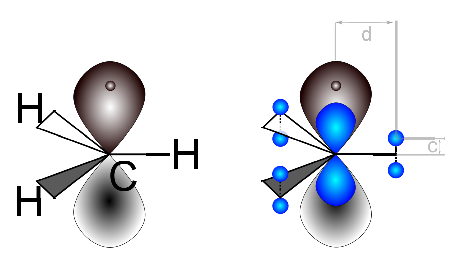
\includegraphics[width=8cm]{scheme_complete.eps}
\end{center}
{\Large
\begin{minipage}[t]{3in}
\baselineskip = .5\baselineskip
Figure 2 \\
Alexander Punter, Paola Nava, Yannick Carissan\\
Int. J. Quantum Chem.
\end{minipage}
}
\end{figure}

\clearpage

\begin{figure}
\begin{center}
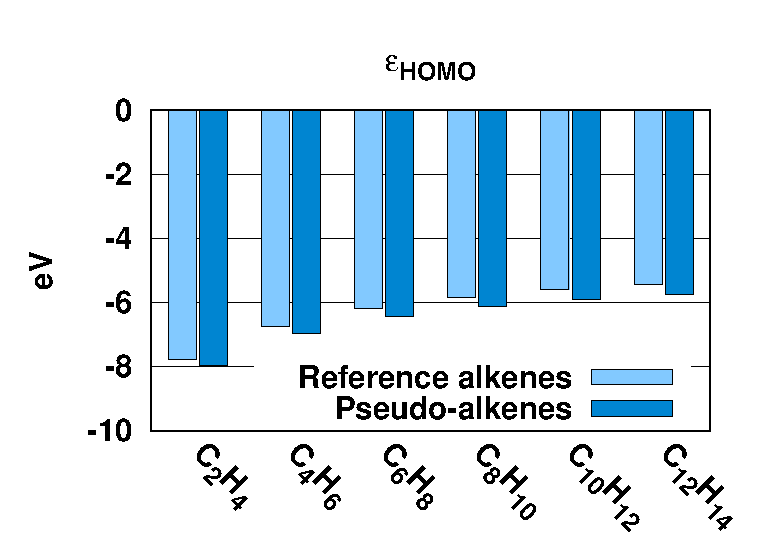
\includegraphics[width=8cm]{short_pbe0_homo_uhf}\\
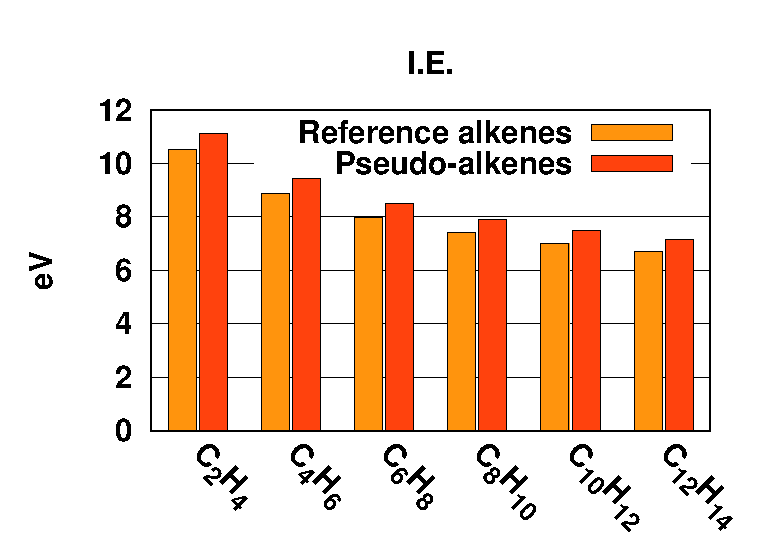
\includegraphics[width=8cm]{short_pbe0_ie_uhf}\\
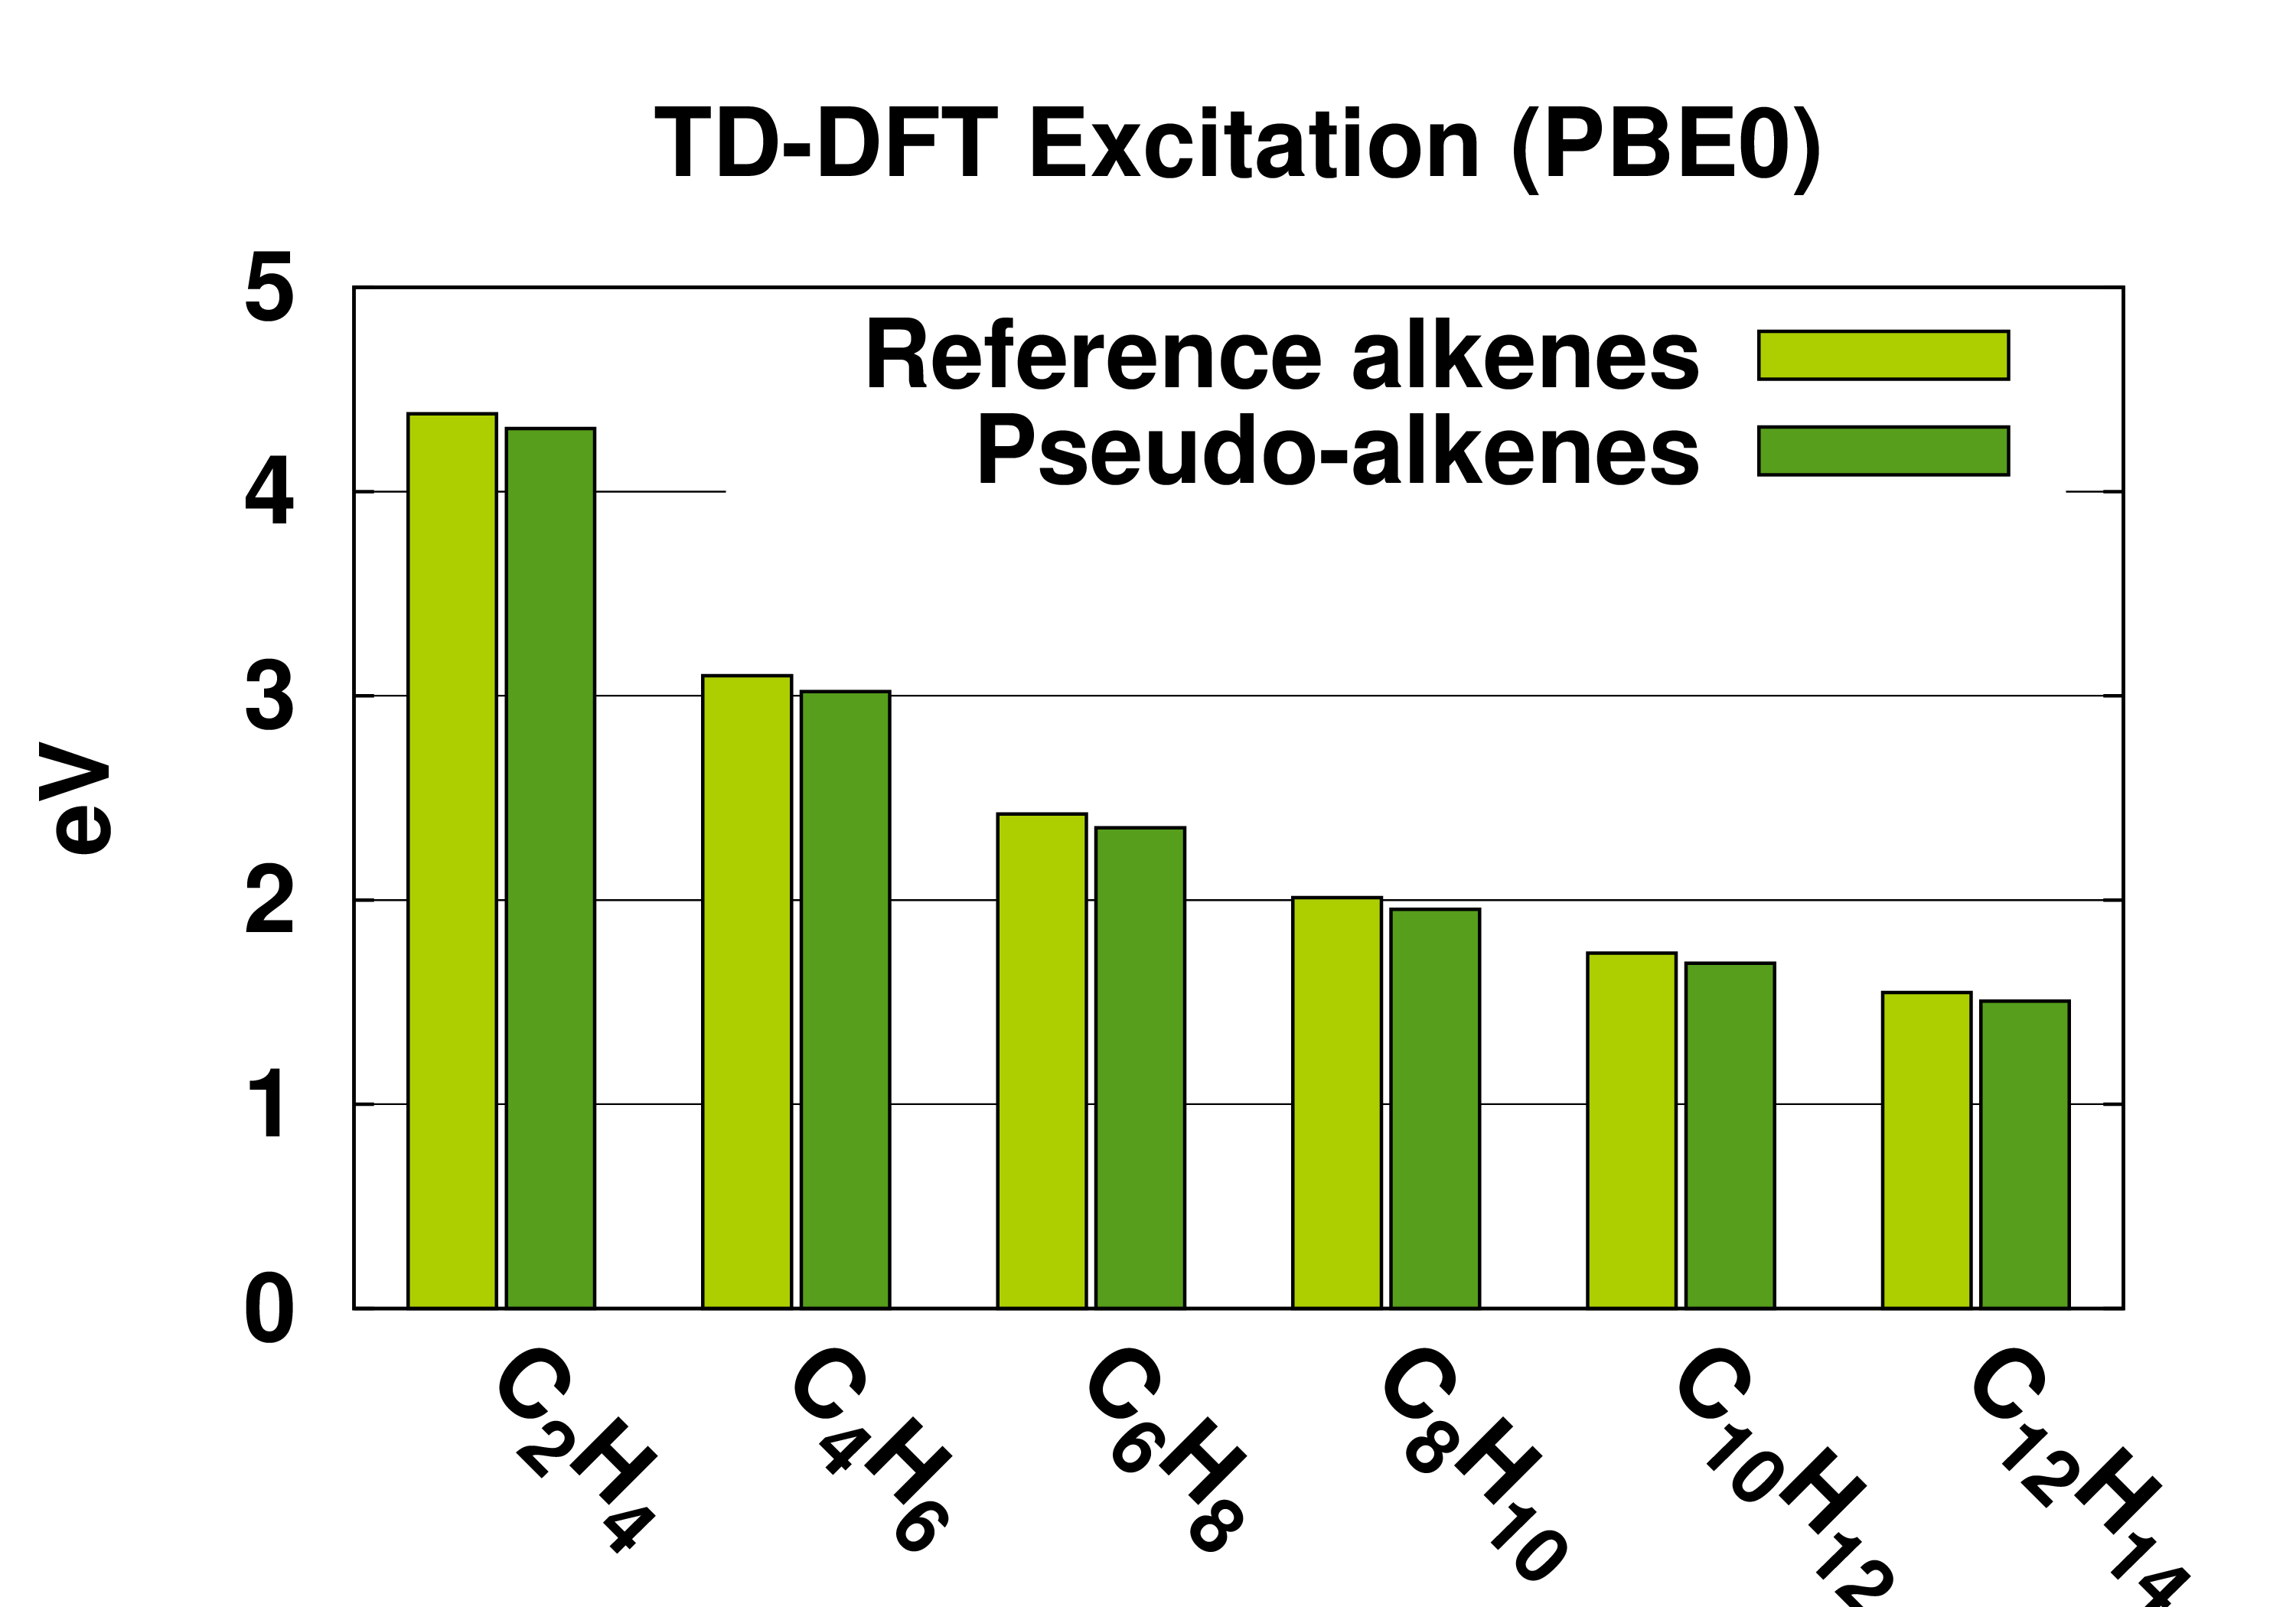
\includegraphics[width=8cm]{short_pbe0_tddft}
\end{center}
{\Large
\begin{minipage}[t]{3in}
\baselineskip = .5\baselineskip
Figure 3 \\
Alexander Punter, Paola Nava, Yannick Carissan\\
Int. J. Quantum Chem.
\end{minipage}
}
\end{figure}

\clearpage

\begin{figure}
\begin{center}
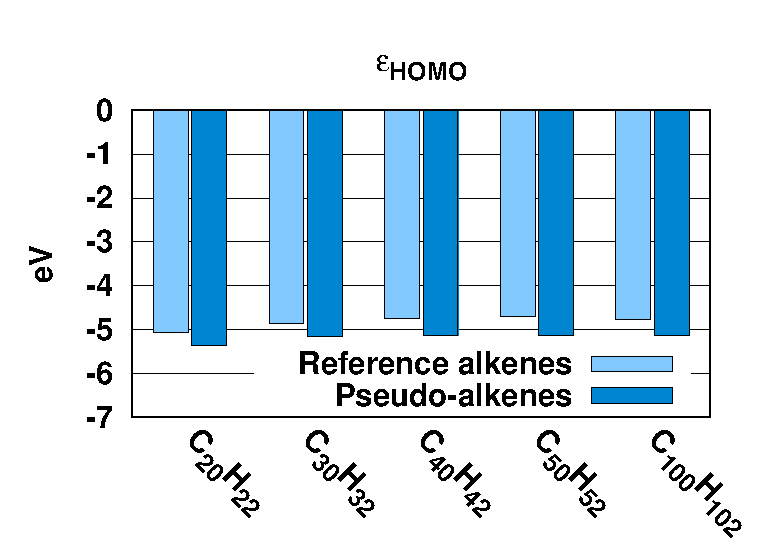
\includegraphics[width=8cm]{long_pbe0_homo_uhf}\\
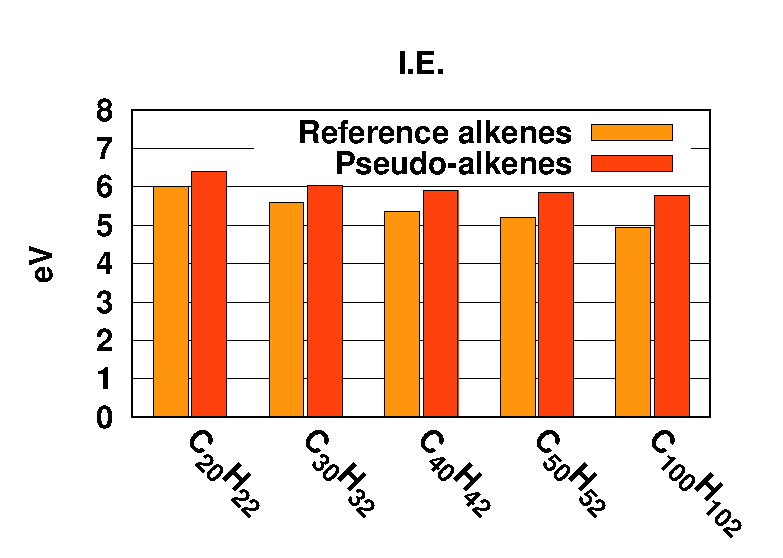
\includegraphics[width=8cm]{long_pbe0_ie_uhf}\\
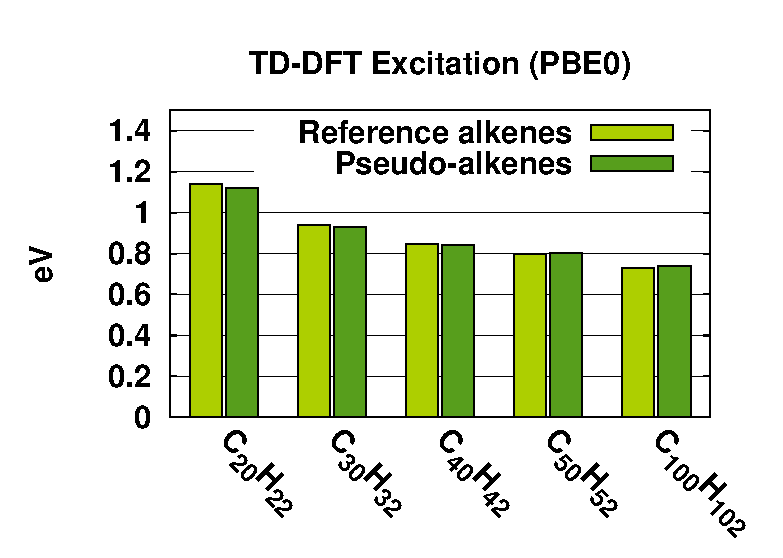
\includegraphics[width=8cm]{long_pbe0_tddft}
\end{center}
{\Large
\begin{minipage}[t]{3in}
\baselineskip = .5\baselineskip
Figure 4 \\
Alexander Punter, Paola Nava, Yannick Carissan\\
Int. J. Quantum Chem.
\end{minipage}
}
\end{figure}

\clearpage

\begin{figure}
\begin{center}
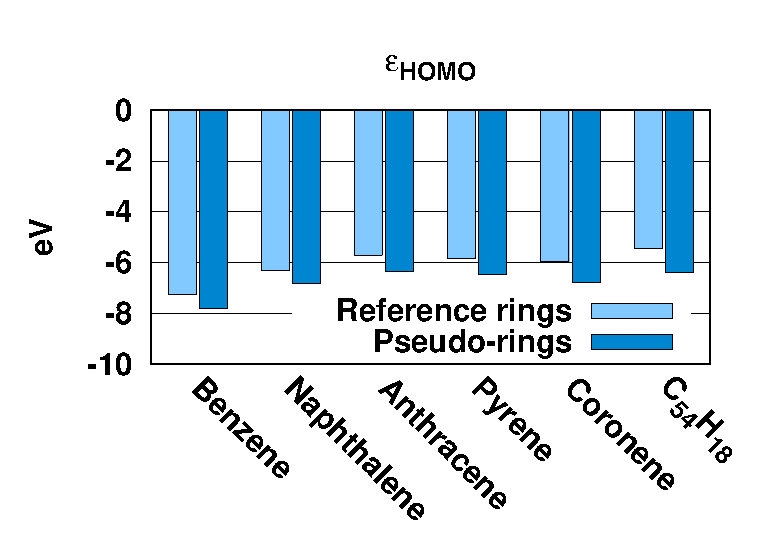
\includegraphics[width=8cm]{ring_pbe0_homo_uhf}\\
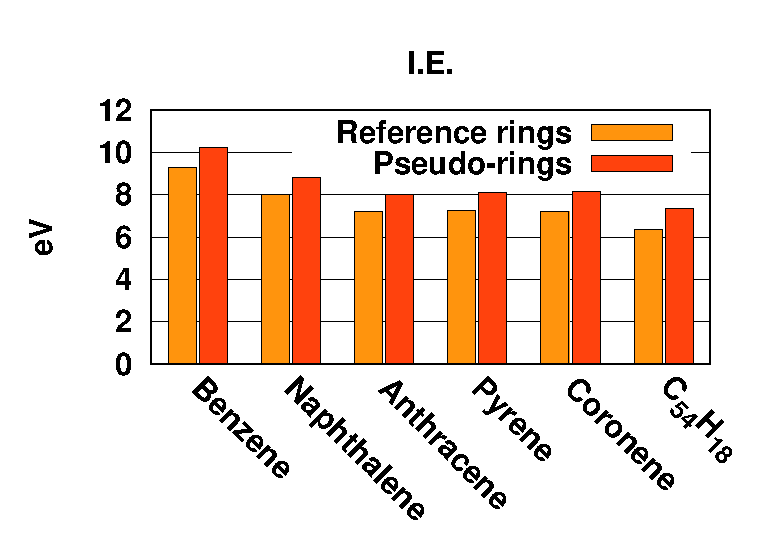
\includegraphics[width=8cm]{ring_pbe0_ie_uhf}\\
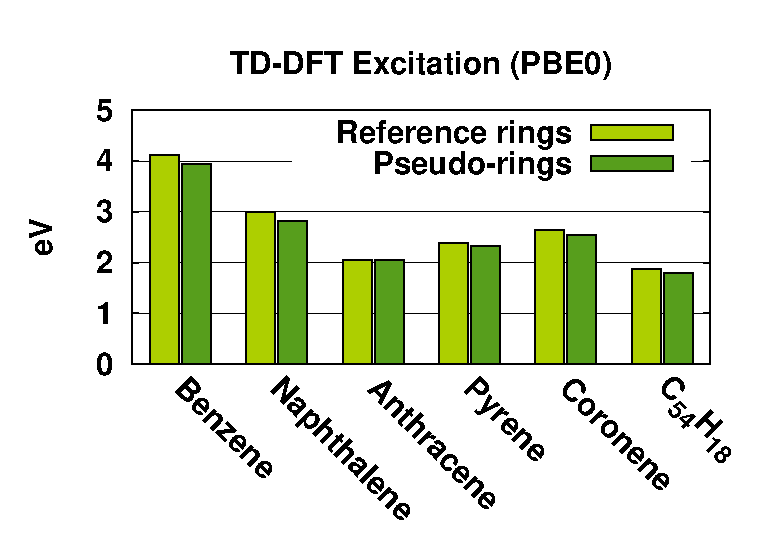
\includegraphics[width=8cm]{ring_pbe0_tddft}\\
\fbox{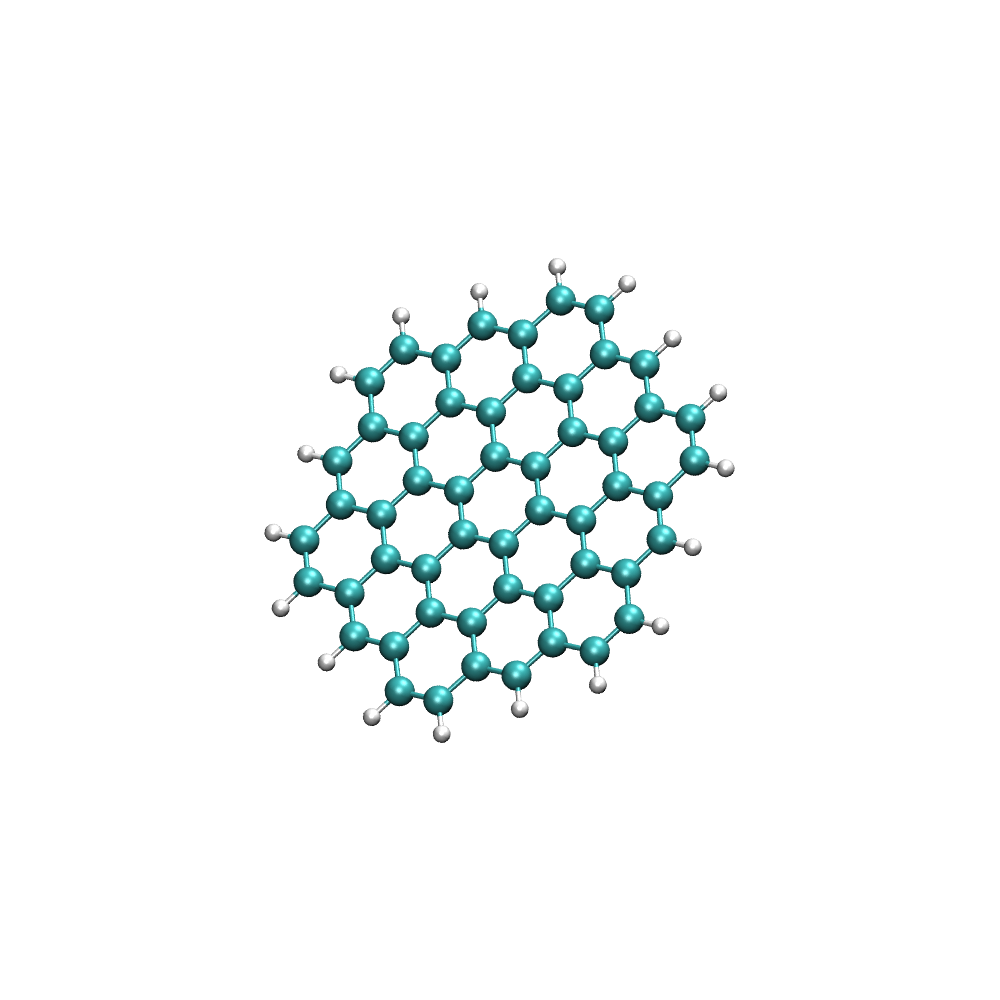
\includegraphics[width=5cm]{c54h18}}
\end{center}
{\Large
\begin{minipage}[t]{3in}
\baselineskip = .5\baselineskip
Figure 5 \\
Alexander Punter, Paola Nava, Yannick Carissan\\
Int. J. Quantum Chem.
\end{minipage}
}
\end{figure}

\clearpage

\begin{figure}

\begin{center}
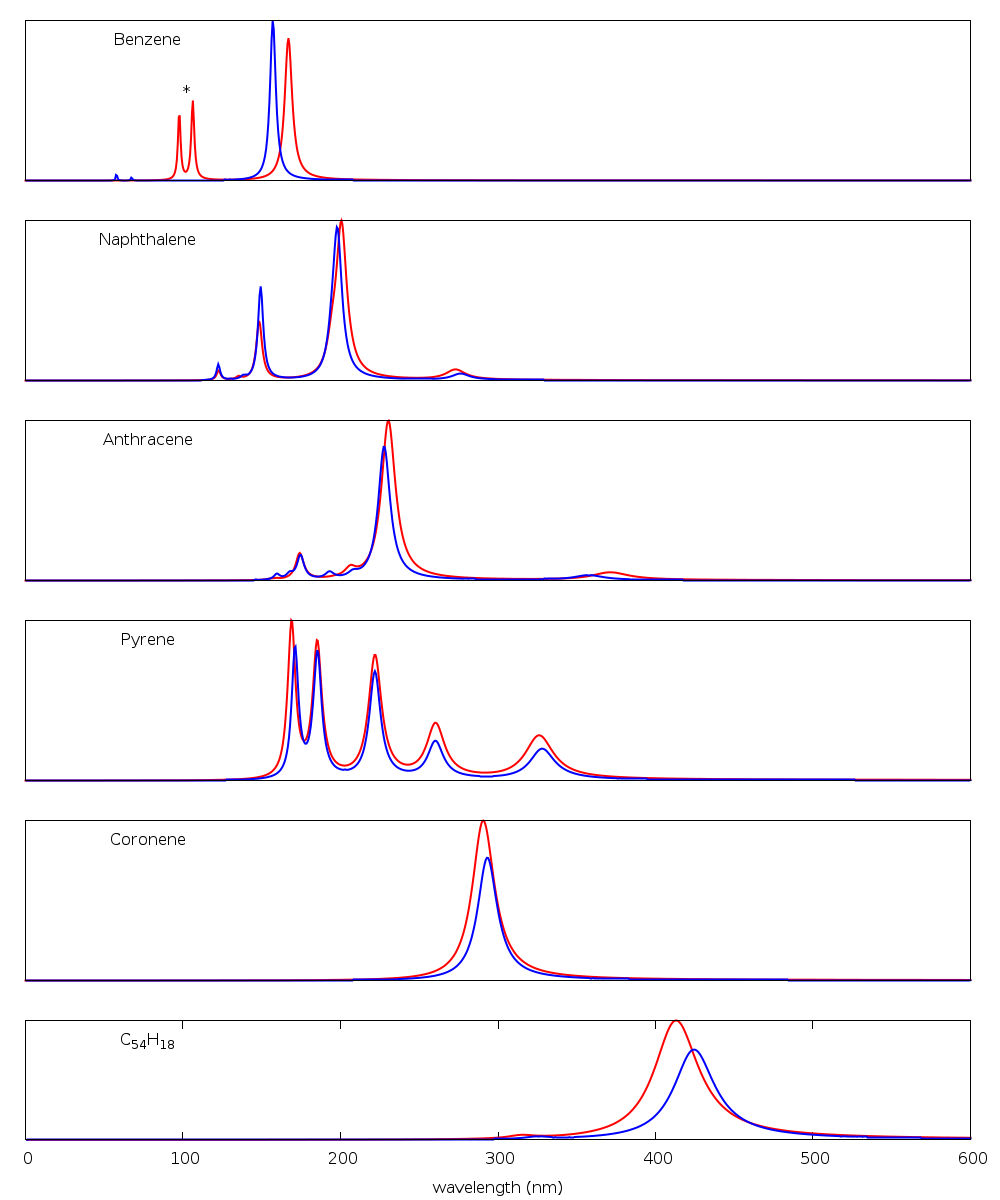
\includegraphics[width=8cm]{grand_rpa_singlet}
\end{center}
{\Large
\begin{minipage}[t]{3in}
\baselineskip = .5\baselineskip
Figure 6 \\
Alexander Punter, Paola Nava, Yannick Carissan\\
Int. J. Quantum Chem.
\end{minipage}
}
\end{figure}

\clearpage

\begin{figure}
\begin{center}
\begin{tabular}{|c|c|}
\hline
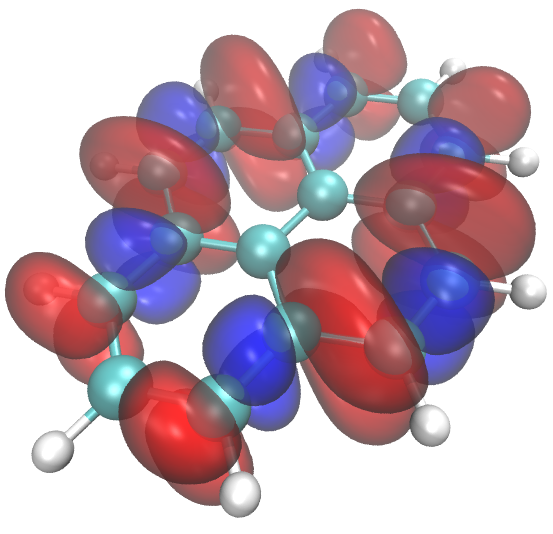
\includegraphics[width=4cm]{pyrene_peak1_ref_white} &
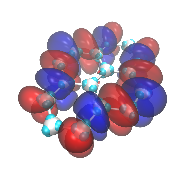
\includegraphics[width=4cm]{pyrene_peak1_ps_white} \\
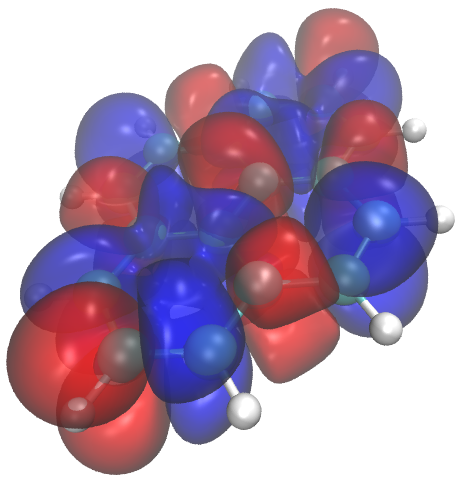
\includegraphics[width=4cm]{pyrene_peak2_ref_white} &
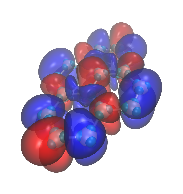
\includegraphics[width=4cm]{pyrene_peak2_ps_white} \\
\hline
All-electron & Pseudo-potential\\
\hline
\end{tabular}\\
\end{center}
\vspace{0.25in}
{\Large
\begin{minipage}[t]{3in}
\baselineskip = .5\baselineskip
Figure 7 \\
Alexander Punter, Paola Nava, Yannick Carissan\\
Int. J. Quantum Chem.
\end{minipage}
}
\end{figure}

\clearpage

\begin{figure}
\begin{center}
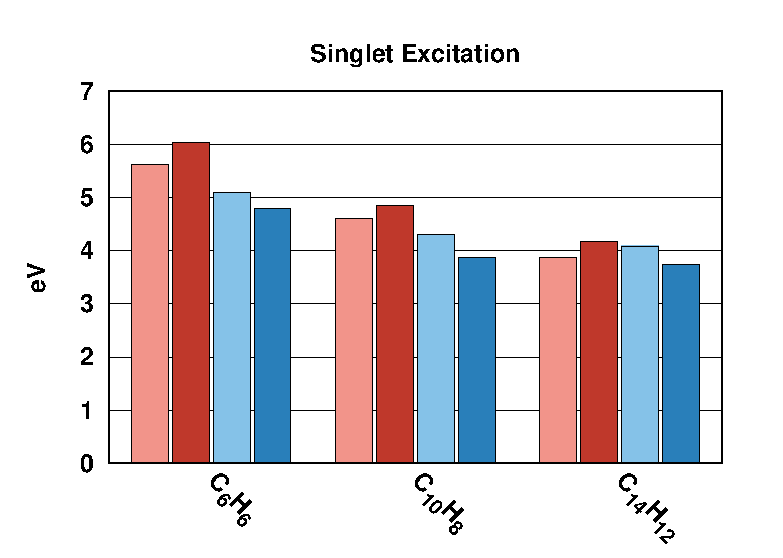
\includegraphics[width=8cm]{methodcomp_s_excitations.eps}\\
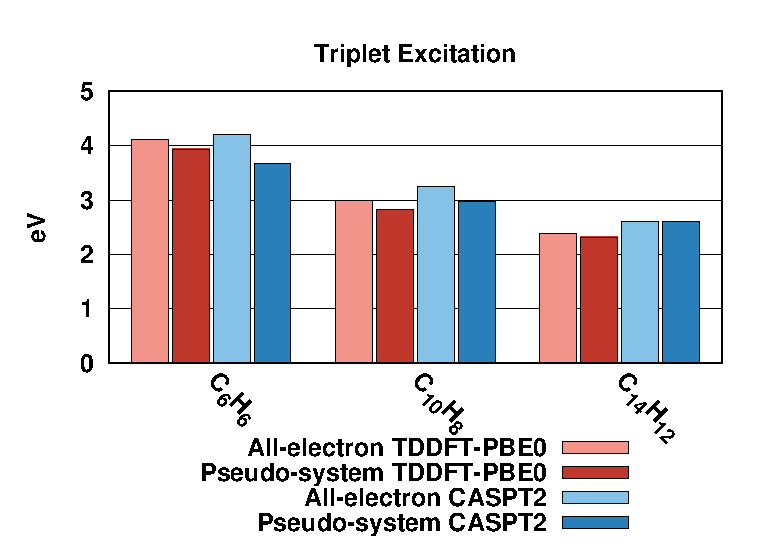
\includegraphics[width=8cm]{methodcomp_t_excitations.eps}\\
\end{center}
{\Large
\begin{minipage}[t]{3in}
\baselineskip = .5\baselineskip
Figure 8 \\
Alexander Punter, Paola Nava, Yannick Carissan\\
Int. J. Quantum Chem.
\end{minipage}
}
\end{figure}

\clearpage

\begin{figure}

\begin{center}
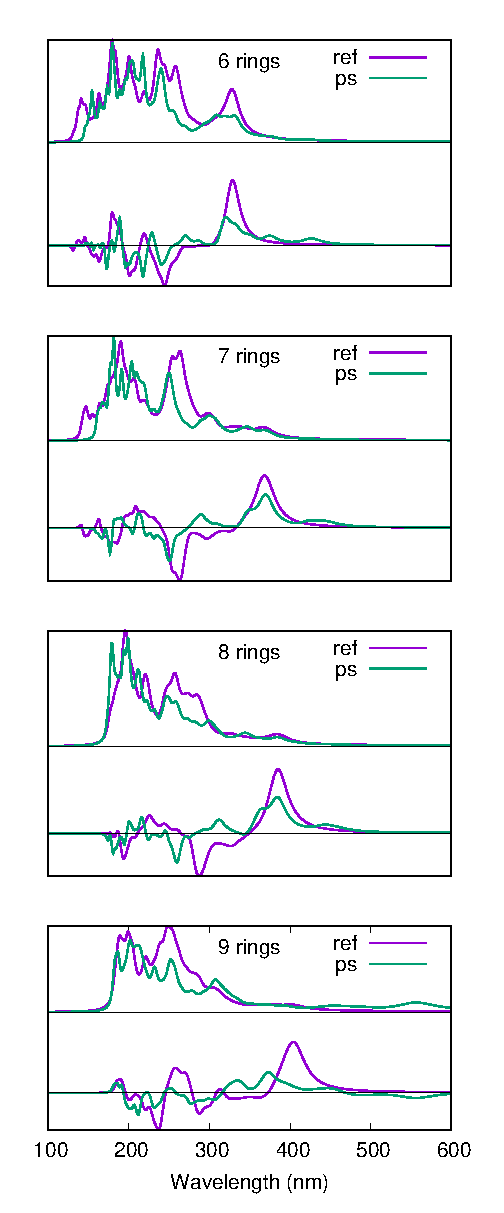
\includegraphics[width=8cm]{helicene_uv_ecd}
\end{center}
{\Large
\begin{minipage}[t]{3in}
\baselineskip = .5\baselineskip
Figure 9 \\
Alexander Punter, Paola Nava, Yannick Carissan\\
Int. J. Quantum Chem.
\end{minipage}
}
\end{figure}

\clearpage

\begin{figure}
\begin{center}
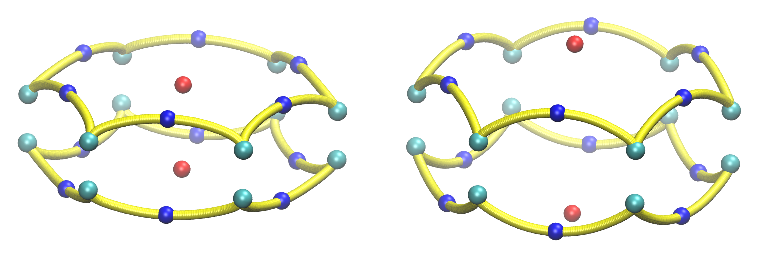
\includegraphics[width=8cm]{aim_c6h6.eps}
\end{center}
{\Large
\begin{minipage}[t]{3in}
\baselineskip = .5\baselineskip
Figure 10 \\
Alexander Punter, Paola Nava, Yannick Carissan\\
Int. J. Quantum Chem.
\end{minipage}
}
\end{figure}

\clearpage

\begin{figure}
\begin{center}
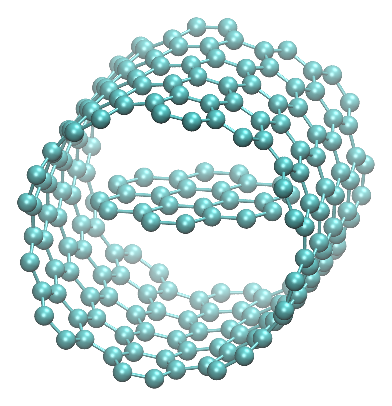
\includegraphics[width=8cm]{nanotube_model_crop.eps}
\end{center}
{\Large
\begin{minipage}[t]{3in}
\baselineskip = .5\baselineskip
Figure 11 \\
Alexander Punter, Paola Nava, Yannick Carissan\\
Int. J. Quantum Chem.
\end{minipage}
}
\end{figure}

\clearpage

\begin{figure}
\begin{center}
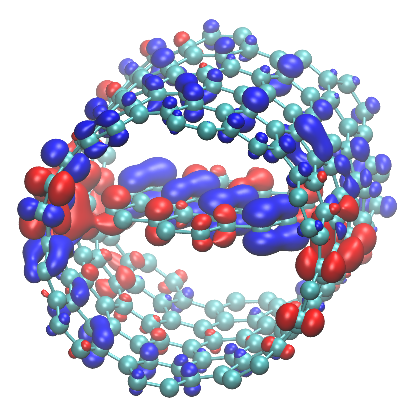
\includegraphics[width=3.8cm]{trans_55_crop.eps}\hspace*{4mm}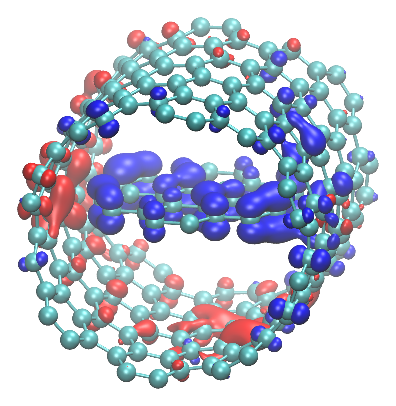
\includegraphics[width=3.8cm]{trans_59_crop.eps}
\end{center}
{\Large
\begin{minipage}[t]{3in}
\baselineskip = .5\baselineskip
Figure 12 \\
Alexander Punter, Paola Nava, Yannick Carissan\\
Int. J. Quantum Chem.
\end{minipage}
}
\end{figure}

\clearpage

\begin{table}[h]
\caption{\label{table:potential_params} Comparison of molecular properties of pseudo-CH$^{\bullet}_{3}$ and pseudo-C$_{2}$H$_{4}$ molecules, along with pseudo-potential parameters and all-electron values (Hartee-Fock level).}
\begin{tabular}{| c | c | c | c | c | c | c | c| }
\hline
 & \multicolumn{2}{c}{\textbf{$\bm{p}$}} & \multicolumn{2}{c|}{$\bm{s}$} & \multicolumn{3}{c|}{\textbf{Energy (eV)}} \\
System & coeff. & exp & coeff. & exp. & HOMO & $\Delta_{ST}$ & 1$^{st}$ Ionisation \\
\hline
ref. CH$^{\bullet}_{3}$ & - & - & - & - & -10.537 & - & - \\
ref. C$_{2}$H$_{4}$ & - & - & - & - & -10.363 & -3.522 & 9.091 \\
\hline
initial pseudo-CH$^{\bullet}_{3}$ & -3.268 & 0.295 & 10.381 & 10.000 & -10.537 & - & - \\
initial pseudo-C$_{2}$H$_{4}$ & -3.268 & 0.295 & 10.381 & 10.000 & -14.061 & -9.214 & 14.021\\
\hline
final pseudo-CH$^{\bullet}_{3}$ & -3.910 & 0.624 & 1.500 & 0.500 & -10.000 & - & - \\
final pseudo-C$_{2}$H$_{4}$ & -3.910 & 0.624 & 1.500 & 0.500 & -10.062 & -3.533 & 9.806 \\
\hline
\end{tabular}
\end{table}


\newpage

\begin{table}[h]
\caption{Errors across calculation types for all-trans-polyenes C$_n$H$_{n+2}$}
\begin{tabular}{|l| c| c| c| c |}
\hline
\textbf{Calculation Type} & \textbf{PBE0} & \textbf{PBE} & \textbf{TPSS} & \textbf{TPSSh} \\
\hline
\multicolumn{5}{|c|}{Short polyenes (n=2,4,6,8,10)}\\
\hline
Mean Ionisation  error (\%) & 7.0 & 8.8 & 11.3 & 9.9 \\\hline
Mean Singlet HOMO  error (\%) & 4.2 & 9.3 & 13.7 & 10.7 \\\hline
Mean TD-DFT Excitation error (\%) & 2.6 & 2.7 & 5.9 & 6.4 \\ 
\hline
\multicolumn{5}{|c|}{Long polyenes (n=20, 30, 40, 50, 100)}\\
\hline
Mean Ionisation  error (\%) & 6.6 & 10.3 & 11.3 & 11.2 \\\hline
Mean Singlet HOMO  error (\%) & 7.8 & 12.8 & 20.1 & 15.7 \\\hline
Mean TD-DFT Excitation error (\%) & 1.0 & 6.8 & 6.1 & 2.9 \\
\hline
\end{tabular}
\label{table:alkene_errors}
\end{table}

\newpage

\begin{table}[h]
\caption{Errors across calculation types for PAH}
\begin{tabular}{|l |c |c |c |c |}
\hline
\textbf{Calculation Type} & \textbf{PBE0} & \textbf{PBE} & \textbf{TPSS} & \textbf{TPSSh} \\
\hline
Mean Ionisation  error (\%) & 12.0 & 15.4 & 18.0 & 16.1 \\\hline
Mean Singlet HOMO  error (\%) & 11.5 & 17.1 & 22.3 & 18.7 \\\hline
Mean TD-DFT Excitation error (\%) & 4.4 & 2.6 & 5.9 & 6.5 \\
\hline
\end{tabular}
\label{table:ring_system_errors}
\end{table}

\newpage
\begin{table}
\caption{\label{tab:coef}Comparison of the weights (all-electron \emph{vs.} pseudo-potentials)
of the excitations obtained with TD-DFT
to represent the triplet excited state from the closed shell singlet state.
Example case of C$_{50}$H$_{52}$.}
\begin{tabular}{|c |c |c |c|}
\hline
\multicolumn{2}{|c|}{\textbf{Excitation}} & \multicolumn{2}{c|}{\textbf{Weight(\%)}}\\
\multicolumn{2}{|c|}{MO} & Ref. & Pseudo.\\
\hline
\multicolumn{2}{|c|}{25 a" \(\rightarrow\) 26 a"} & 77.0 &   67.1  \\\hline
\multicolumn{2}{|c|}{24 a" \(\rightarrow\) 27 a"} & 10.5 &   13.1  \\\hline
\multicolumn{2}{|c|}{23 a" \(\rightarrow\) 28 a"} & 3.6  &    5.2  \\
\hline
\end{tabular}
\end{table}
%ENDTAB

\begin{table}[ht]
\caption{\label{tab:time}Time (in seconds) per SCF iteration and relative
gain (time ratio all-electron/pseudo-potential) for a standard and a large basis set.} 
\begin{tabular}{|l|r|r|}
\hline
\textbf{Model}            & \textbf{def2-SV(P)} & \textbf{QZVPPD} \\
\hline
All electrons    &        67 & 68928 \\\hline
Pseudo-potential &        28 &  8566 \\\hline
Gain (no unit)   &       2.4 &   8.0 \\
\hline
\end{tabular}
\end{table}

\end{document}

